\section{Architecture général du projet}

MDSE fournit des langages appropriés pour définir les transformations de
modèles afin de fournir aux concepteurs des solutions optimisées pour
spécifier les règles de transformation. Ces langages peuvent être
utilisés pour définir des transformations de modèle en termes de modèles
de transformation qui sont généralement appliqués sur des modèles selon
certaines règles de correspondance vérifiées sur des éléments de modèle.
Ces règles de transformation peuvent être définies selon différentes
approches : la transformation peut être écrite manuellement à partir de
zéro par un développeur, ou peut être défini comme une spécification
raffinée d'une spécification existante. Alternativement, les
transformations elles-mêmes peuvent être produites automatiquement à
partir de certaines règles de mappage de niveau supérieur entre les
modèles. Le schema suivant résume l'architecture générale de cette
technique.

\section{Description du meta-model JDL}

Le définition des meta Model du JDL et YAML fait référence à la création
d'une abstraction permettant de décrire les modèles. Ainsi, La création
d'une application sous Jhispter nécessite la configuration à 
travers un fichier avec un format specific en YAML, qui'en résulte
des valeur attribué à des champs spécifiques dans un fichier JDL. 
Ces champs doivent être obligatoirement présente dans la conception
du meta-modèle.

\section{Description du meta-model JDL}

La figure suivante présente un diagramme de classe décrivant 
le meta Model du JDL:

% \begin{figure}[H]
%   \begin{center}
%       \fbox{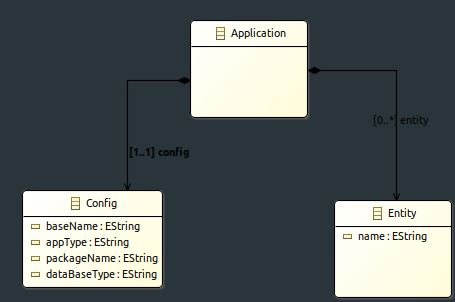
\includegraphics[width=16cm]{mmJdl.png}}
%       \caption{}
%   \end{center}
% \end{figure}

\subsection{Description du meta-model YAML}

La figure suivante présente un diagramme de classe décrivant 
le meta Model du YAML:

Aussi pour YAML:\\
\begin{figure}[H]
  \begin{center}
      \fbox{
      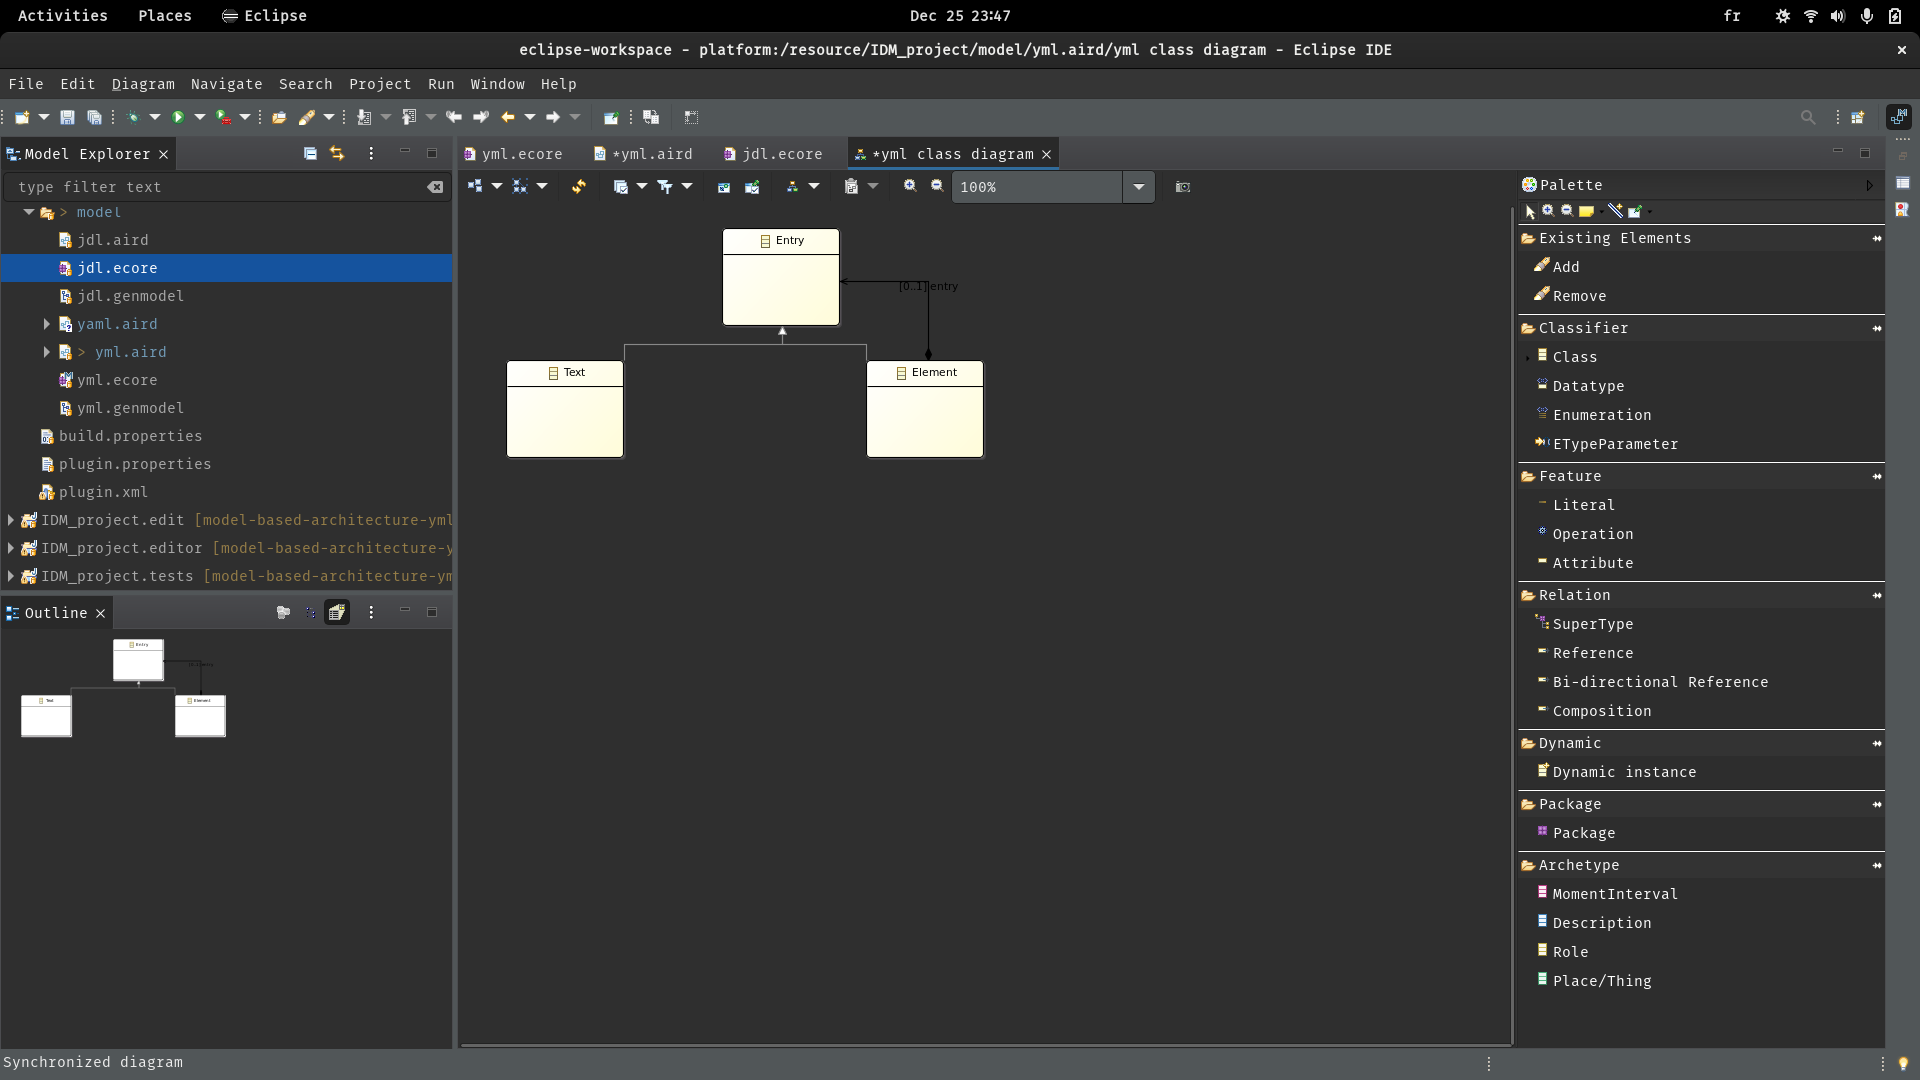
\includegraphics[width=16cm]{eclipse_yaml.png}
      }
      \caption{}
  \end{center}
\end{figure}